% Drop-in figure environments. Paths are relative to paper/.
% Each graphic is 7.0 in wide. In this manuscript \linewidth is about 6.5 in,
% so width=\linewidth scales the type down by about 7 percent.
% Minimum drawn type is 6.2 pt, which remains above 5.7 pt at that scale;
% the labels that carry counts are 6.6--8 pt.

\begin{figure}[t]
\centering
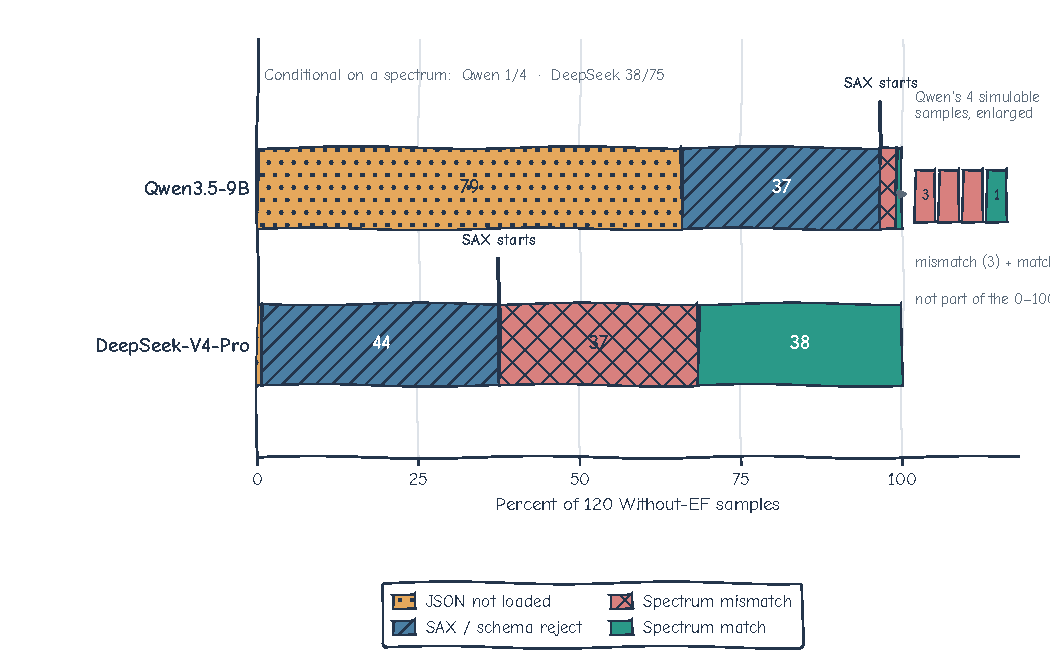
\includegraphics[width=\linewidth]{../paper_figures/fig1_failure_audit.pdf}
\caption{A simulable netlist is not a spectrum match.
Each bar is one Without-EF sample, and the four stages are mutually exclusive.
JSON not loaded joins a missing result span to a \texttt{json.loads} rejection:
7+72 for Qwen3.5-9B and 1+0 for DeepSeek-V4-Pro.
SAX / schema rejection is a parsed object the simulator does not accept
(Qwen: runtime 25, model name 9, ports 3; DeepSeek: 12, 8, and 24).
The navy tick is the first sample SAX can simulate.
Syntax pass is the coral segment plus the teal segment: 4 and 75.
Functional pass is the teal segment alone: 1 and 38.
The four cells at the right repeat Qwen's simulable samples at equal width
and are marked enlarged; they are not part of the 0--120 axis.
Counts are Table~\ref{tab:loci}.}
\label{fig:failure-audit}
\end{figure}

\begin{figure}[t]
\centering
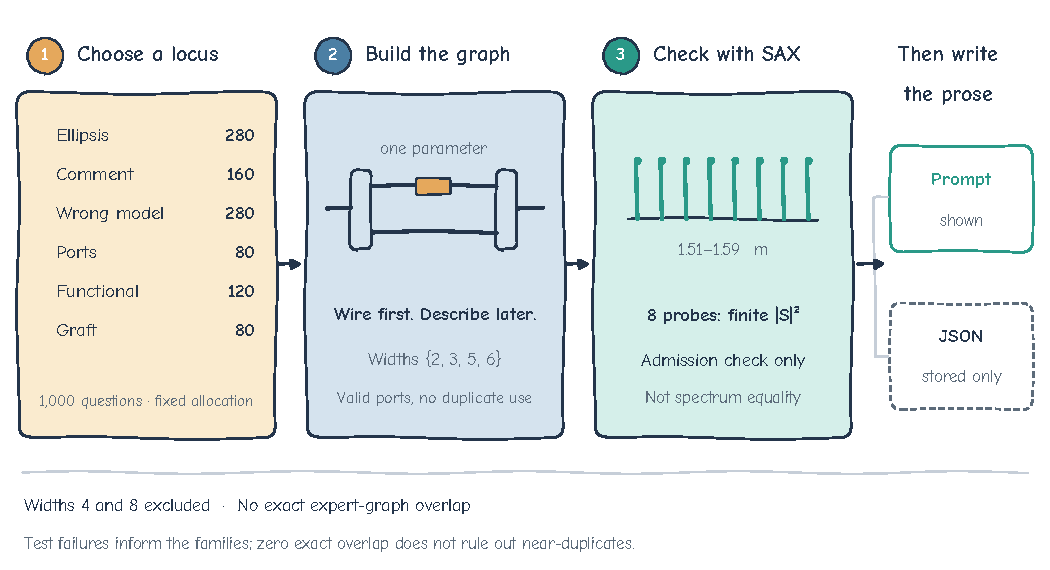
\includegraphics[width=\linewidth]{../paper_figures/fig2_failure_verbalization.pdf}
\caption{Failure-locus verbalization builds the circuit before the prose.
The six weights are a manual allocation from an earlier text heuristic
(280, 160, 280, 80, 120, 80), not a fit to the re-audit in Table~\ref{tab:loci}.
The schematics are the constructions those loci use.
They are not the 24 expert netlists, and the eight stems are not a device spectrum:
admission keeps a draw only when \(|S|^2\) is finite on eight wavelengths.
The 1{,}000-point equality test is a different check, used later on teacher replies and on PICBench.
The prompt receives the natural-language specification.
The reference JSON is stored and is not shown to the model.
Widths 4 and 8 are held out; sampled widths are \(\{2,3,5,6\}\);
the 24 expert problems are excluded from generation.
Exact structural-fingerprint overlap with those 24 graphs is 0.
That screen does not rule out softer leakage.}
\label{fig:verbalization-redesign}
\end{figure}

\begin{figure}[t]
\centering
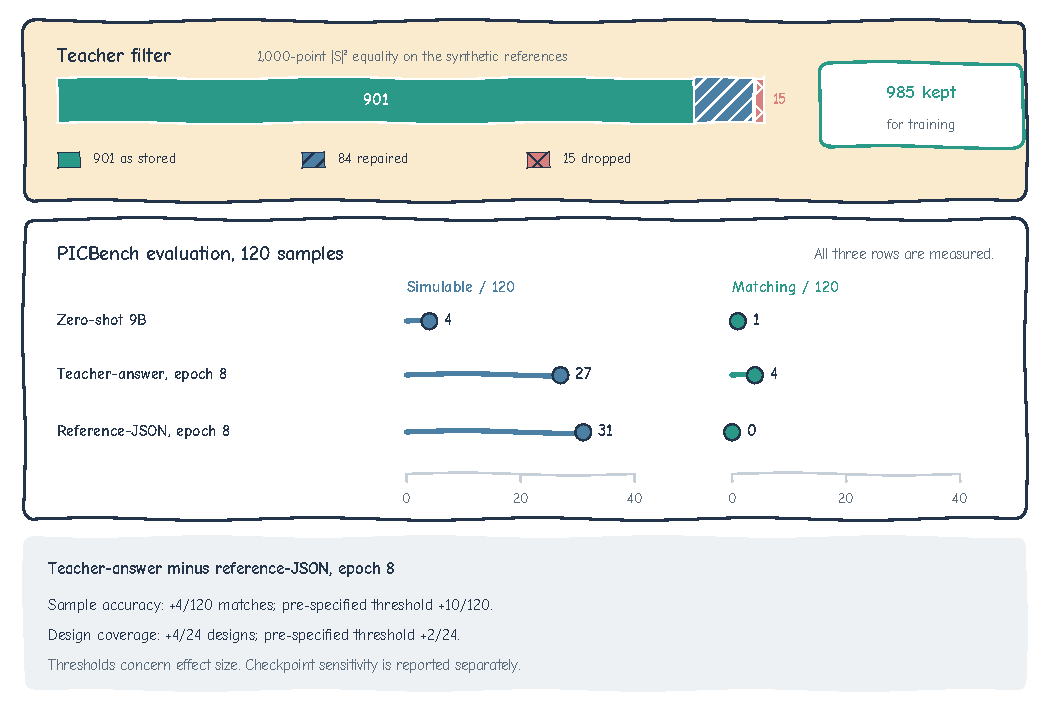
\includegraphics[width=\linewidth]{../paper_figures/fig3_teacher_sft.pdf}
\caption{Executability moved. The $10/120$ functional bar was not cleared.
Of 1{,}000 teacher replies, 901 match the synthetic reference on the 1{,}000-point grid as stored,
84 match after an identity model-name repair, and 15 do not match and are dropped.
The training file keeps 985.
Student marks are counts out of 120 on one shared 0--40 scale.
Reference-JSON epoch 8 has 31 simulable netlists and 0 matches; teacher-answer epoch 8 has 27 and 4.
The functional gap is $4/120$, below $10/120$.
The design-count gap is $4/24$, above the separate $2/24$ bar.
Neither bar is a significance test.}
\label{fig:teacher-boundary}
\end{figure}

\begin{figure}[t]
\centering
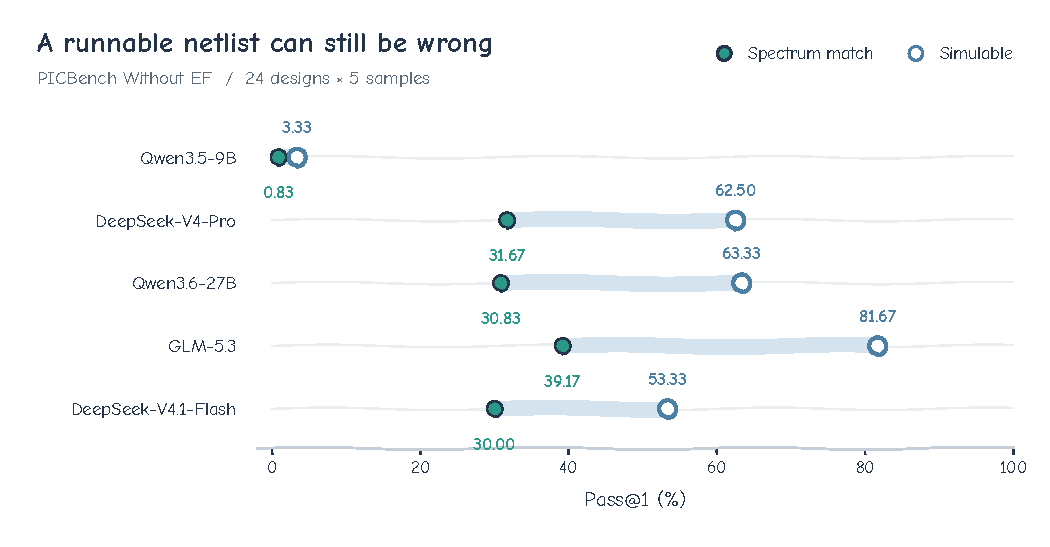
\includegraphics[width=\linewidth]{../paper_figures/fig4_syntax_function_gap.pdf}
\caption{Syntax and functional $\mathrm{Pass@}1$ for the five models measured here.
Syntax includes functional matches, so the segment between the dots is the
rate of simulable netlists whose spectrum misses the expert file.
The four API models fall between 30.00 and 39.17 functional $\mathrm{Pass@}1$,
while syntax $\mathrm{Pass@}1$ spans 53.33 to 81.67.
Vertical order follows Table~\ref{tab:published}.
It is not a scale ranking: deployment, size, and reasoning configuration are not held fixed.
The transcribed rows of that table were not redrawn.}
\label{fig:pass1-gap}
\end{figure}
